% include the figures path relative to the master file
\graphicspath{ {./content/method/figures/} }

\section{\uppercase{Balancing strategies}}\label{sec:met}

\noindent Considering a binary classification problem, the class with the smallest number of samples is defined as the \textit{minority} class and its counterpart is defined as the \textit{majority} class.
The problem of data balancing corresponds to equalize the number of samples of both the minority and majority classes. This task can be achieved in either data or feature space.

\begin{figure*}
  \hspace*{\fill}
  \subfloat[][]{
    \label{fig:GridOriginal}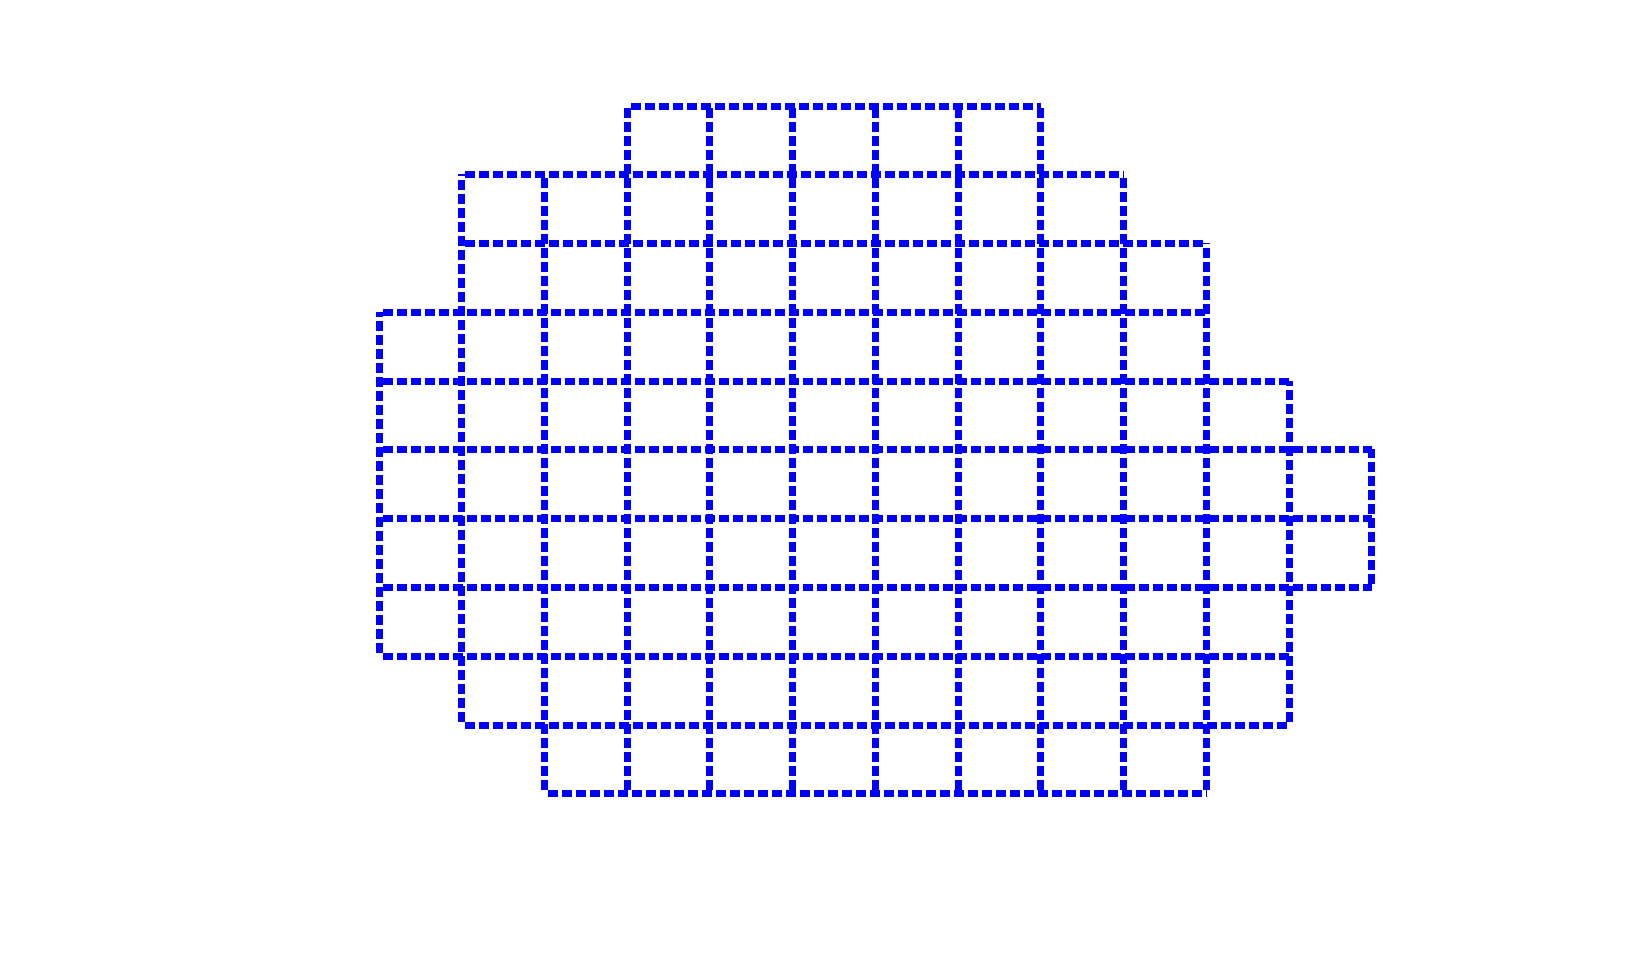
\includegraphics[width=0.3\textwidth]{OG.png}}\hfill
  \subfloat[][]{
    \label{fig:GridGaussian}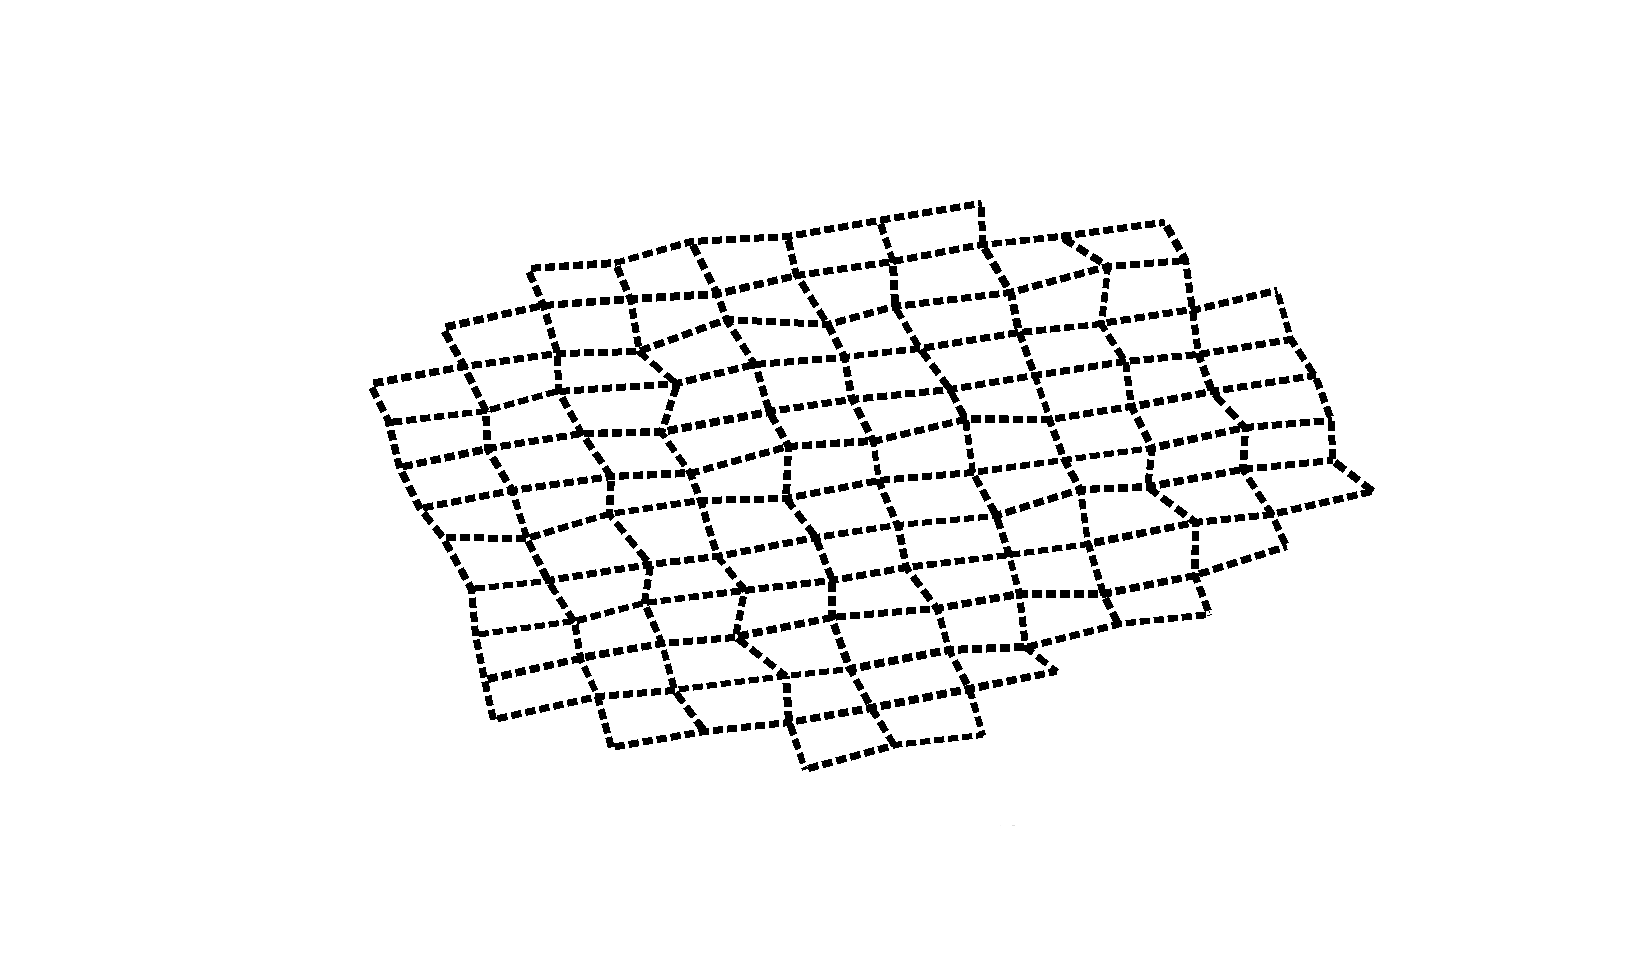
\includegraphics[width=0.3\textwidth]{GG3_80.png}}\hfill
  \subfloat[][]{
    \label{fig:GridBarrel}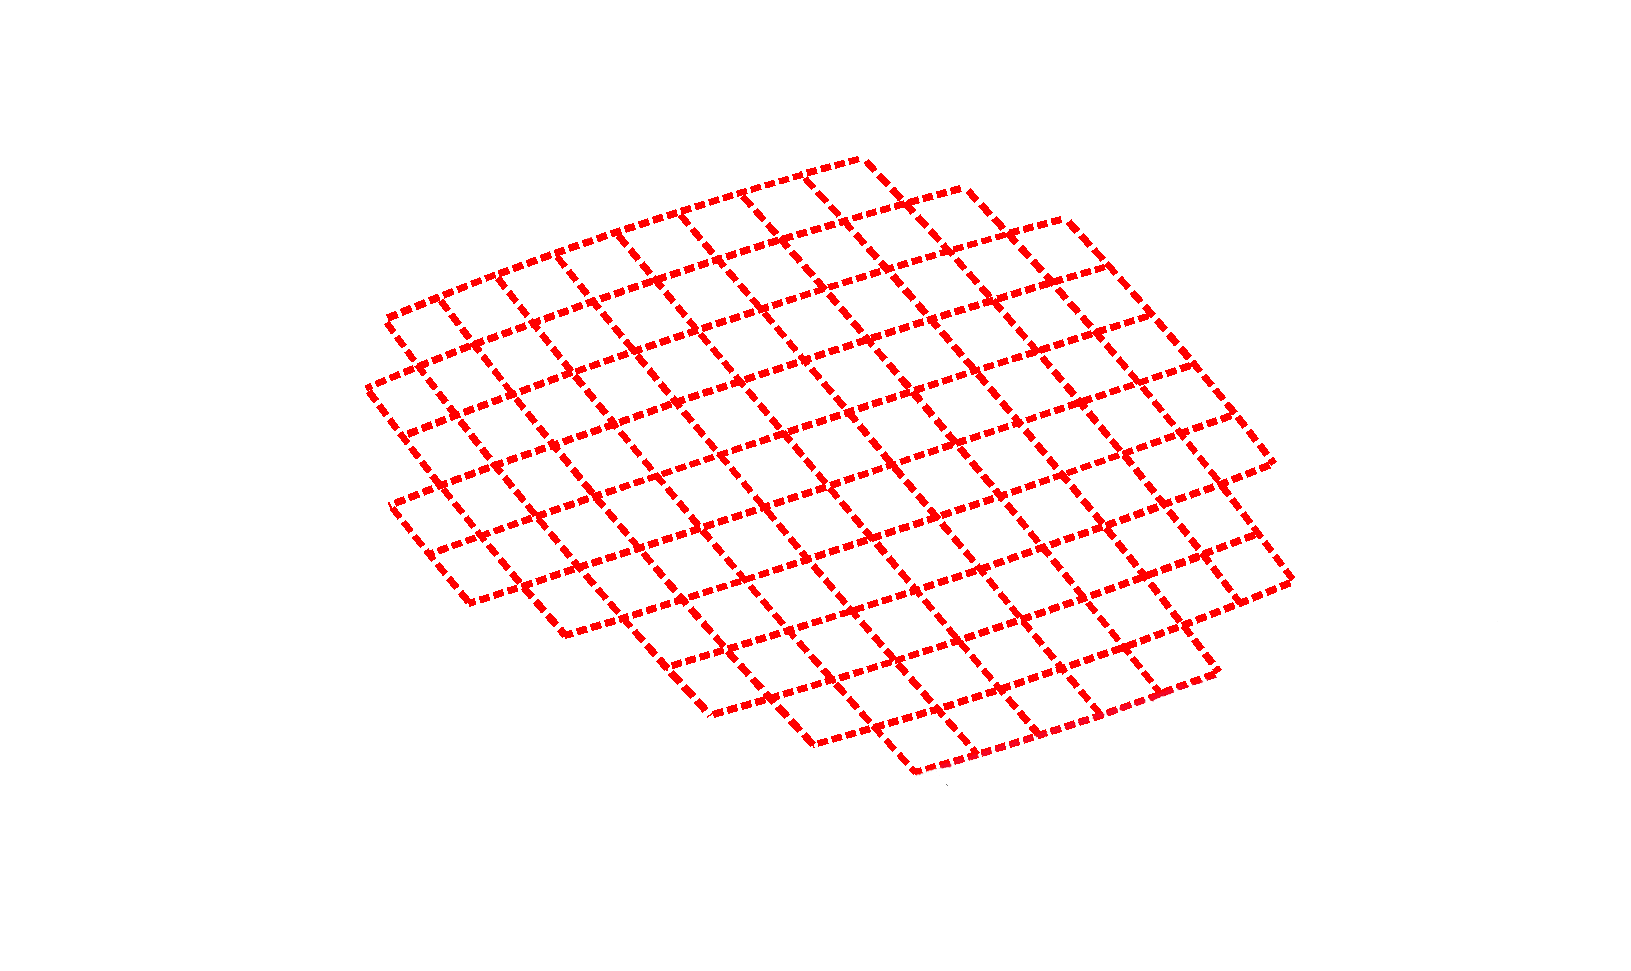
\includegraphics[width=0.3\textwidth]{BG3_145.png}}
  \hspace*{\fill}
  \caption{Data space transformation: \protect\subref{fig:GridOriginal} original synthetic data, \protect\subref{fig:GridGaussian} \acs*{rdgm} deformation, \protect\subref{fig:GridBarrel} \acs*{bd} deformation.}
  \label{fig:DSOS}
\end{figure*}


\subsection{Data space sampling}

Data space sampling is related with the generation of new synthetic samples by modifying the original data ahead of any feature extraction processes. 
\Ac{os} is performed on the original dataset by generating synthetic melanoma images based on two types of deformation~\cite{rastgoo2015ensemble}. Furthermore, cubic b-spline interpolation is used with both methods to approximate non-integer points in the image.
These deformations are considered since they are more likely to occur, due to un-flatten surface of some body parts, skin wrinkles, camera rotation, and position. 
%Different rotations and barrel deformation are considered to account for camera rotation and body un-flatten surfaces. 
%The \ac{rdgm} deformation with specific Gaussian criteria is considered to account for acceptable amount of wrinkles.

 
\begin{description}
	\item[\Ac{rdgm}] achieved by deforming the original image by adding a random Gaussian motion $\mathcal{N}(\mu, \sigma) = (0,5)$ at each pixel compounded with a global rotation of~\SI{80}{\degree}.
	\item[\Ac{bd}] corresponds to a deformation of the original image using barrel distortion compounded with a global rotation of~\SI{145}{\degree}.
\end{description}
A synthetic example illustrating the results of these deformation is presented in Fig.\,\ref{fig:DSOS}.

\subsection{Feature space sampling}

Three strategies can be employed to overcome the problem of imbalanced dataset: (i) \ac{us}, (ii) \ac{os}, and (iii) a combination of both.
The following sections give an overview of the techniques used to tackle this issue.

\subsubsection{\acl{us}}

Considering the problem of imbalanced, \ac{us} is performed such that the number of samples of the majority class is reduced to be equal to the number of samples of the minority class.
The following methods are considered to perform such balancing.


\begin{description}
  \item[\Ac{rus}] is performed by randomly selecting without replacement a subset of samples from the majority class such that the number of samples is then equal in both minority and majority classes.
  \item[\Ac{tl}] can be used to under-sample the majority class of the original dataset~\cite{tomek1976two}.
Let define a pair of \ac{nn} samples $(x_i, x_j)$ such that their associated class label $y_i \neq y_j$.
The pair $(x_i, x_j)$ is defined as a \ac{tl} if, by relaxing the class label differentiation constraint, there is no other sample $x_k$ defined as the \ac{nn} of either $x_i$ or $x_j$.
\Ac{us} is performed by removing the samples belonging to the majority class and forming a \ac{tl}.
It can be noted that this \ac{us} strategy does not enforce a strict balancing between the majority and the minority classes.
  \item[\Ac{cus}] refers to the use of a $k$-means to cluster the feature space such that $k$ is set to be equal to the number of samples composing the minority class.
Hence, the centroids of these clusters define the new samples of the majority class. 
  \item[\Ac{nm}] offers three different methods to under-sample the majority class~\cite{mani2003knn}.
In \ac{nm1}, samples from the majority class are selected such that for each sample, the average distance to the $k$ \ac{nn} samples from the minority class is minimum.
\ac{nm2} diverges from \ac{nm1} by considering the $k$ farthest neighbours samples from the minority class.
In \ac{nm3}, a subset $M$ containing samples from the majority class is generated by finding the $m$ \ac{nn} from each sample of the minority class.
Then, samples from the subset $M$ are selected such that for each sample, the average distance to the $k$ \ac{nn} samples from the minority class is maximum.
In our experiment, $k$ and $m$ are fixed to 3.
  \item[\Ac{ncr}] consists of applying two rules depending on the class of each sample~\cite{laurikkala2001improving}.
Let define $x_i$ as a sample of the dataset with its associated class label $y_i$.
Let define $y_m$ as the class of the majority vote of the $k$ \ac{nn} of the sample $x_i$.
If $y_i$ corresponds to the majority class and $y_i \neq y_m$, $x_i$ is rejected from the final subset.
If $y_i$ corresponds to the minority class and and $y_i \neq y_m$, then the $k$ \ac{nn} are rejected from the final subset.
\end{description}

\subsubsection{\acl{os}}

\noindent In the contrary, the data balancing can be performed by \ac{os} in which the new samples belonging to the minority class are generated aiming at equalizing the number of samples in both classes.
Two different methods are considered.

\begin{description}
\item[\Ac{ros}] is performed by randomly replicating the samples of the minority class such that the number of samples is equal in both minority and majority classes.
\end{description}

\include*{content/method/framework-result-ls}

\begin{description}
\item[\Ac{smote}] is a method to generate synthetic samples in the feature space~\cite{chawla2002smote}.
Let define $x_i$ as a sample belonging to the minority class.
Let define $x_{nn}$ as a randomly selected sample from the $k$ \ac{nn} of $x_i$.
Therefore, a new sample $x_j$ is generated such that $x_j = x_i + \sigma \left( x_{nn} - x_i \right)$, where $\sigma$ is a random number in the interval $\left[0,1\right]$.
\end{description}

\begin{table*}[ht]
\caption{The classification costs, $C$ for different balancing techniques and feature sets.}
\centering
\resizebox{1.\textwidth}{!}{
\begin{tabular}{l ccc ccc ccc}
\toprule
%Features &  \multicolumn{3}{l}{Color}& \multicolumn{3}{l}{Texture} & \multicolumn{3}{l}{Combined}\\
%  \cmidrule(r){2-4}  \cmidrule(r){5-7}  \cmidrule(r){8-10}  
 Balancing techniques & \multicolumn{9}{c}{Classification cost, $C$} \\\cmidrule{2-10}
		   & \multicolumn{1}{c}{$C_{1}$}& \multicolumn{1}{c}{$C_{2}$}& \multicolumn{1}{c}{$C_{1,2}$}& \multicolumn{1}{c}{$T_{1}$} &  \multicolumn{1}{c}{$T_{2}$} & \multicolumn{1}{c}{$T_{1,2}$}& \multicolumn{1}{c}{$T_{1},C_{1,2}$}& \multicolumn{1}{c}{$T_{2},C_{1,2}$}& \multicolumn{1}{c}{$T_{1,2},C_{1,2}$}\\ 
  \midrule 
IB& 						0.3267 			&  0.1950 			& 0.2225 		& 0.4008 			& 0.2550   & 0.2275 			& 0.1992 		  & 0.2142 			& 0.2025\\
\midrule \midrule
\ac{os}&   				\cellcolor[gray]{0.6}0.1708 &  0.1750    		& 0.1567    		& 0.4025    			&\cellcolor[gray]{0.6}0.2050   & 0.2133 			& 0.1867  		  & 0.1592 			& 0.1742\\
\midrule \midrule
\ac{os}&					0.3467 			&  0.1833 			& 0.2233  		& 0.4167 			& 0.2833   & 0.2508 			& 0.2083 		  & 0.2125 			& 0.2142\\
\ac{smote}&				0.3100  			&  0.1892  			& 0.2133   		& 0.3658   			& 0.2825   & 0.2317  		& 0.1875 		  & 0.2192 			& 0.2175\\
\hdashline \noalign{\vskip 3pt}
\ac{rus}&				0.2733 			&  0.1625   			& 0.2075   		& 0.3817   			& 0.2375   & 0.1750  		& 0.1525  		  & 0.1750 			& 0.1317\\
\ac{tl}&					0.3475  			&  0.1908   			& 0.2417   		& 0.4233   			& 0.2483   & 0.2208  		& 0.2025  		  & 0.2575 			& 0.2000\\
\ac{cus}&				0.2408  			&  0.1817   			& 0.1608   		& 0.3992   			& 0.2700   & 0.1817  		& 0.1725  		  & 0.1833 			& 0.1658\\
\ac{nm1}& 				0.3067  			&  0.1658   			& 0.1600   		& 0.3900   			& 0.2700   & 0.2083  		& 0.1617   		  & 0.1608 			& 0.1517\\
\ac{nm2}& 				0.2883  			&  0.1575   			& 0.1583   		& 0.3475   			& 0.3192   & 0.2775  		& \cellcolor[gray]{0.6}0.1467 &\cellcolor[gray]{0.6}0.1350  &\cellcolor[gray]{0.6}0.1258\\
\ac{nm3}& 				0.2050  			&  0.1517   			& 0.1683   		& 0.3342   			& 0.2350   & 0.1833  		& 0.1725  		  & 0.1700  			& 0.1608\\
\ac{ncr}& 				0.2958  			& \cellcolor[gray]{0.6}0.1500  & 0.1617   		& 0.3233   			& 0.2067   &\cellcolor[gray]{0.6}0.1717  & 0.1558  		  & 0.1650  			& 0.1558\\
\hdashline \noalign{\vskip 3pt}
\ac{smote}+\acs*{enn}& 	0.2492  			&  0.1650   			& 0.1617   		&\cellcolor[gray]{0.6}0.2875    & 0.2142   & 0.2017  		& 0.1575  		  & 0.1675  			& 0.1958\\
\ac{smote}+\ac{tl}& 		0.2550 			&  0.1675   			&\cellcolor[gray]{0.6}0.1517 & 0.3283   		    & 0.2067   & 0.2125  		& 0.1617  		  & 0.2033  			& 0.1375\\
\bottomrule
\end{tabular}
}
\label{tab:tab2}
\end{table*}

\subsubsection{Combination of \ac{os} and \ac{us}}

\noindent Subsequently, \ac{os} methods can be combined with \ac{us} methods to clean the subset created.
In that regard, two different combinations are tested.

\begin{description}
  \item[\ac{smote} + \ac{tl}] are combined to clean the samples created using \ac{smote}~\cite{batista2003balancing}.
\ac{smote} over-sampling can lead to overfitting which can be avoided by removing the \ac{tl} from both majority and minority classes~\cite{prati2009data}.
  \item[\ac{smote} + \ac{enn}] are combined for the same aforementioned reason~\cite{batista2004study}.
\end{description}

\section{\uppercase{Classification}}
\label{sec:clas-val}

\noindent The classification is performed using a \ac{rf} classifier.
\Ac{rf} is an ensemble of decision trees~\cite{breiman2001random} which generalizes the classification process by applying two types of randomization: at the tree level, each tree is fed by a bootstrap made of $S'$ samples built from the original data of size $S$ such that  $S=S'$, and at the node level, a subset of feature dimensions $m$ is randomly selected from the original dimension $M$ such that $m=\sqrt{M}$. 
The trees in \ac{rf} are grown to their maximum length without any pruning.
Each tree in the ensemble casts a unit vote in the final prediction and the final prediction is based on combination of all the votes. 
\Ac{rf} is used with 100 un-pruned trees and the original feature dimension of size $M=\{144,84,228,26,48,74,254,276,302\}$

\subsection{Validation}
We used a 10-fold cross-validation scheme to validate our classifier with stratified sampling.
However, differently from the usual 10-fold cross-validation, 8 folds were kept for training and 2 folds for testing at each iteration. 
The training set is balanced using previously described imbalanced techniques. 
The classification performance are reported in terms of average \ac{se}~(TPR) and \ac{sp}~(TNR) over 10 runs of cross-validation. 
The visual and analytic interpretation of these evaluation measures are depicted in Fig.\,\ref{fig:evaluation}.

The best performance is selected based on the cost function defining the trade off between \ac{se} and \ac{sp} as in \cite{barata2013towards}, which is formulated as:
\begin{equation}\label{eq:cost}
C = \frac{c_{10}(1-\ac{se})+c_{01}(1-\ac{sp})}{c_{10}+c_{01}} \ ,
\end{equation}
\noindent where, $c_{10}$ and $c_{01}$ are the costs of incorrectly classifying a melanoma and non-melanoma lesions, respectively.
In cancer classification such as melanoma, correctly identifying the cancer lesions has high importance (i.e., high \ac{se}). 
Thus incorrect classification of melanoma is not desired and $c_{10}$ is a greater error and evidently more costly and should be penalized more. 
In order to achieve a high \ac{se} without significantly reducing the value of \ac{sp}, Barata~\emph{et al.} proposed to set $c_{10} = 1.5 \times c_{01}$ and $c_{01} = 1$~\cite{barata2013towards}.  
We considered the same configuration for our cost function. 

\colorlet{circle edge}{blue!50}
\colorlet{circle area}{blue!20}


% Definition of circles
% \def\myRadius{1.5cm}
% \def\vennSpace{(0,0) rectangle (6cm,4cm)}
% \def\predictedCircle{(2cm,2cm) circle (\myRadius)}
% \def\actualCircle{(4cm,2cm) circle (\myRadius)}
% \def\myLabelRadius{1.3cm}

\def\myRadius{.75cm}
\def\vennSpace{(0,0) rectangle (3cm,2cm)}
\def\predictedCircle{(1cm,1cm) circle (\myRadius)}
\def\actualCircle{(2cm,1cm) circle (\myRadius)}
\def\myLabelRadius{.60cm}

\tikzset{fillbase/.style={fill=circle area, draw=circle edge, thick},
         filled/.style={pattern=crosshatch dots, draw=circle edge, thick},
         outline/.style={draw=circle edge, thick}}

\def\drawPredicted{
    \draw[outline] \predictedCircle node (x){}; % {$\bullet$};
    \node [above left=\myLabelRadius of x, anchor=center, outer sep=0](p){$P$};
    \node  at (p.300) {$+$};
    \node  at (p.120) {$-$};
}

\def\drawActual{
    \draw[outline] \actualCircle node (x){}; % {$\bullet$};
    \node [above right=\myLabelRadius of x, anchor=center, outer sep=0](a){$A$};
    \node  at (a.60) {$-$};
    \node  at (a.240) {$+$};
}

% Define the different metrics: tp, tn, fp, fn
\def\tp{
      \draw[outline] \vennSpace;
      \begin{scope}
        \clip \predictedCircle;
        \fill[filled] \actualCircle;
      \end{scope}
      \drawPredicted
      \drawActual
      % \draw[outline] (current bounding box.south west)
      %   rectangle (current bounding box.north east);
}

\def\tn{
      \draw[outline] \vennSpace;
  \begin{scope}[even odd rule]
    \fill[filled] \vennSpace
      \actualCircle
      \predictedCircle;
    \clip \actualCircle;
    \fill[white] \predictedCircle;
  \end{scope}
  \drawPredicted
  \drawActual
}

\def\fp{
      \draw[outline] \vennSpace;
      \begin{scope}
        \clip \predictedCircle;
        \fill[filled, even odd rule]
              \predictedCircle \actualCircle;
      \end{scope}
      \draw[outline] \vennSpace;
      \drawPredicted
      \drawActual
}

\def\fn{
      \draw[outline] \vennSpace;
      \begin{scope}
        \clip \actualCircle;
        \fill[filled, even odd rule]
              \actualCircle \predictedCircle;
      \end{scope}
      \draw[outline] \vennSpace;
      \drawPredicted
      \drawActual
}

\def\se{
  \fill[fillbase] \actualCircle;
      \begin{scope}
        \clip \predictedCircle;
        \fill[filled] \actualCircle;
      \end{scope}
      \draw[outline] \vennSpace;
      \drawPredicted
      \drawActual
}


\def\sp{
  \fill[fillbase, even odd rule]
    \vennSpace \actualCircle;
  \begin{scope}[even odd rule]
    \fill[filled] \vennSpace
      \actualCircle
      \predictedCircle;
    \clip \actualCircle;
    \fill[white] \predictedCircle;
  \end{scope}
  \draw[outline] \vennSpace;
  \drawPredicted
  \drawActual
  }


\begin{figure}

  \def\myRadius{.65cm}
  \def\vennSpace{(0,0) rectangle (2.6cm,1.6cm)}
  \def\predictedCircle{(.8cm,.8cm) circle (\myRadius)}
  \def\actualCircle{(1.8cm,.8cm) circle (\myRadius)}
  \def\myLabelRadius{.450cm}

  \subfloat[][Confusion matrix with truly and falsely positive samples detected (TP, FP) in the first row, from left to right and the falsely and truly negative samples detected (FN, TN) in the second row, from left to right.]{
    \label{fig:evaluation:confusion_matrix}
    \begin{tikzpicture}[scale=0.5]
      \node at (0,0){
        \begin{tabular}{
            >{\centering}m{1em} >{\centering}m{1em} >{\centering}m{1in} >{\centering\arraybackslash}m{1in}}
          % c>{\centering}m{2em}ccc}
          & & \multicolumn{2}{c}{ Actual Class }\\
          & & A+ & A- \\
          % \parbox[t]{2mm}{\multirow{2}{*}{\rotatebox[origin=c]{90}{\usebox \centering Predicted Class}}}& P+ &  \tikz{\tp} & \tikz{\fp} \\
          \multirow{3}{*}{\rotatebox[origin=c]{90}{Predicted Class}}& P+ &  \tikz{\tp} & \tikz{\fp} \\
          & P- & \tikz{\fn} & \tikz{\tn}
        \end{tabular}
      };
    \end{tikzpicture}
  }\\
  \centering
  \subfloat[][\acl*{se} and \acl*{sp} evaluation, corresponding to the ratio of the doted area over the blue area.]{
    \label{fig:evaluation:roc_axis}
    \begin{tikzpicture}[scale=0.5]
      \def\seEquation{$SE = \frac{TP}{TP+FN}$}
      \def\spEquation{$SP = \frac{TN}{TN+FP}$}
      \node[label={[]below:\seEquation}](se){\tikz{\se}};
      \node[right=5pt of se, label={[]below:\spEquation}]{\tikz{\sp}};
      % \node[label={[]right:\seEquation}](se){\tikz{\se}};
      % \node[below=5pt of se, label={[]right:\spEquation}]{\tikz{\sp}};
    \end{tikzpicture}
  }

  \caption{Evaluation metrics:
    \protect\subref{fig:evaluation:confusion_matrix} confusion matrix,
    \protect\subref{fig:evaluation:roc_axis} \acl*{se} - \acl*{sp}
  }
  \label{fig:evaluation}
\end{figure} 

%%% Local Variables: 
%%% mode: latex
%%% TeX-master: "../../master"
%%% End: 
